\documentclass[aspectratio=169,11pt]{beamer}
\usepackage[T1]{fontenc}
\usepackage{lmodern,booktabs,tikz,amsmath}
\usetikzlibrary{arrows.meta,positioning,calc}
\definecolor{navy}{HTML}{142B45}
\definecolor{slate}{HTML}{536779}
\definecolor{gold}{HTML}{AB802E}
\setbeamercolor{normal text}{fg=navy,bg=white}
\setbeamercolor{frametitle}{fg=navy}
\setbeamercolor{structure}{fg=gold}
\setbeamerfont{frametitle}{size=\Large,series=\bfseries}
\setbeamertemplate{navigation symbols}{}
\setbeamersize{text margin left=9mm,text margin right=9mm}
\setbeamertemplate{frametitle}{\vspace{3mm}\insertframetitle\par\vspace{1mm}{\color{gold}\rule{14mm}{0.7pt}}}
\setbeamertemplate{footline}{\hspace{9mm}\scriptsize\color{slate}SCA / WORKING PAPER\hfill\insertframenumber\hspace{9mm}\vspace{3mm}}
\newcommand{\src}[1]{\par\vspace{1mm}{\fontsize{7}{8.5}\selectfont\color{slate}#1\par}}
\newcommand{\pauseq}[1]{\par\vspace{2.5mm}{\color{gold}\textbf{Pause}}\quad #1\par}
\newcommand{\bigline}[1]{{\Large #1}\par\vspace{3mm}}
\setlength{\parskip}{1.6mm}
\begin{document}

\begin{frame}{Synthetic Cultural Agents from Aggregate Anchors}
\vspace{1mm}
{\large Augusto Gonzalez-Bonorino\quad Kseniia Biriukova\quad Monica Capra}
\vspace{2mm}

{\color{slate}\small Arizona State University \quad/\quad EconLLM Lab \quad/\quad Claremont Graduate University}
\vfill
\bigline{Can a sign-labeled adapter score a new survey item?}
{\color{gold}Working-paper discussion\quad /\quad 16 September 2026}
\end{frame}

\begin{frame}{Background}
SCA 1.0 used cultural descriptions and persona-style prompting, and compared synthetic play to published tables from small-scale society experiments.

This paper changes the supplied information. Public GPS country $z$-scores become sign labels on a shared synthetic pair bank. One joint adapter per country is fitted with DPO. Evaluation prompts omit country names.

The lineage is simulation $\rightarrow$ an inspectable construction. We do not yet claim to have identified a preference parameter or a culture.
\src{SCA 1.0: Capra, Gonzalez-Bonorino, and Pantoja. GPS: Falk et al.\ 2018. This draft: September 2026.}
\end{frame}

\begin{frame}{How much can simulation do on its own?}
\bigline{Human observations remain necessary. The open question is how many, and for what.}
Prompted synthetic respondents mix the researcher's instructions with associations the model already has. That is useful for exploration. It is a weak basis for claiming that an item tracks a preference across populations.

A later human pilot is still the measurement step. The instrument we are discussing is a cheap preliminary readout whose value has to be tested.
\src{Introduction and Discussion. Pre-pilot usefulness is prospective.}
\end{frame}

\begin{frame}{Problems documented, and the scope of this draft}
Persona prompts and other inference-time strategies have many free knobs and mix several effects. Construct validity is then hard to audit. Most social-science uses of these models are about groups, while LLM-generated microdata are poorly understood. Human microdata remain expensive.

\textbf{Scope.} Synthetic comparisons; population-moment anchors; one DPO adapter per group, QLoRA, as a regularized Bradley--Terry pairwise choice fit.

\textbf{Application.} Transport between GPS anchors and WVS item text, compared with a country-named prompt. The question to keep in view: can the adapters score new survey items?
\src{Revised paper §§1--2. No broad priority claim versus CultureLLM, Cao et al., SubPOP, or Jung and Kim.}
\end{frame}

\begin{frame}{Main research questions}
\leavevmode\textcolor{gold}{\textbf{1}}\quad Construction. Can we write an inspectable map from declared aggregate signs, through a shared pair bank, to a fitted scoring policy?

\textcolor{gold}{\textbf{2}}\quad Transport. On held-out WVS text, with no country name in the prompt, do those policies retain GPS country order?

\textcolor{gold}{\textbf{3}}\quad Agreement. Do they match WVS country orderings, and does that depend on the proposed item map?
\src{Claim ladder: construction we have; compiler identification we do not; criterion association on trust order is partial.}
\end{frame}

\begin{frame}{From anchors to a synthetic dataset}
Let $z\in\mathbb{R}^K$ collect $K$ population moments. A labeling map sends $z$ to a dataset of scenarios and opposing responses,
\[
\mathcal{D}=\bigl\{(x,\,y^{+},\,y^{-})\bigr\}.
\]
$x$ is a scenario. $y^{+}$ is written to load high on a target facet; $y^{-}$ to load low. Those loadings are generator judgments.

This first application cares about country \emph{order}. The production map is the sign rule $s_k=1\{z_k\ge 0\}$. Chosen $=A$ when the target coordinate is non-negative, and $B$ otherwise. Magnitudes are stored and later used as the GPS ranking in Spearman. They do not weight the DPO pairs.
\src{Revised paper §3.1. $K=6$: trust, risk, patience, altruism, positive reciprocity, negative reciprocity.}
\end{frame}

\begin{frame}{A sign profile is the construction unit}
\textbf{Argentina:}\quad $(-,\, +,\, -,\, +,\, +,\, -)$
{\small trust / risk / patience / altruism / pos.\ recip.\ / neg.\ recip.}

The United States is non-negative on all six coordinates, so every pair is labeled chosen~A. Mexico is negative on all six, so every pair is labeled chosen~B. That contrast is a global polarity flip of the same 658 scenarios.

16 countries yield 13 distinct sign profiles. Twins share a labeling problem: Mexico--Russia, India--Greece, Indonesia--Egypt.
\pauseq{How should we use the twins as a robustness check?}
\src{If two adapters with the same $s$ diverge on WVS, $\pi$ is not a function of $s$ alone. That test is unrun.}
\end{frame}

\begin{frame}{We replaced an LLM selector with the sign rule}
The teacher and generator still write the shared $A$/$B$ bank. An early labeling path asked a second model to pick $A$ or $B$ given a prose profile.

That selector was instructed that sign sets the direction. On the USA--Mexico checkpoint it matched the sign rule on 1,314 of 1,316 labels. The two misses are Mexico patience at $z=-0.11$.

Production labeling is therefore deterministic. Profile prose is unused. The 16 adapters train on $\mathrm{sign}(z)$ only. The switch was to stop paying a model to re-implement a declared rule with noise.
\src{Relabel run \texttt{gps\_sign\_relabel\_all\_20260816}. Default CLI: \texttt{deterministic\_sign}.}
\end{frame}

\begin{frame}{DPO fits the labeled contests}
\[
\Pr(y_w\succ y_\ell\mid x)=\sigma\!\left(\beta\left[\log\frac{\pi_\theta(y_w\mid x)}{\pi_{\mathrm{ref}}(y_w\mid x)}-\log\frac{\pi_\theta(y_\ell\mid x)}{\pi_{\mathrm{ref}}(y_\ell\mid x)}\right]\right)
\]
The loss raises the chosen text over the rejected text, relative to Llama 3.1 8B. The prompt-specific constant in the implicit reward cancels. This is a contest probability between two texts. It is not $\pi(y_w\mid x)$, and it is not the WVS code softmax.

USA: 658/658 chosen~$A$. Mexico: 658/658 chosen~$B$. The loss pushes $\sigma(\beta\Delta)$ toward 1 as a global polarity. Argentina is mixed: 328 $A$ and 330 $B$, by target dimension. One joint adapter has to implement that patchwork.
\src{Revised paper §3.2. $\beta=0.1$, LoRA rank 16, one epoch, 526/132 split. Notebook settings.}
\end{frame}

\begin{frame}{We fit the whole bank jointly}
All six signs enter the same QLoRA. A trust-item movement is therefore not an isolated trust-bit effect. Countries that differ on GPS trust also differ on other signs. Generator pairs load off-target facets.

What we can report is dimension-specific \emph{transport}: on a named WVS map, do policy country ranks track that GPS $z$. What we cannot report is a ceteris paribus effect of one coordinate.

Llama 3.1 8B is retained because prompted survey simulation is known to be weak there. The test is whether a weight-embedded sign rule survives where a country name in the prompt is a poor instrument.
\src{Revised paper §3.1. Per-dimension adapters are a later object.}
\end{frame}

\begin{frame}{Evaluation surface}
Sixteen purposive countries from the 42-country GPS--WVS intersection, chosen under compute constraints. Twenty-three single-choice WVS items on common support. Same recodes and aggregation across arms.

Egypt was not asked Q69--Q71; Britain was not asked Q174; those items are out everywhere. Patience Q43 and Q50 are scored separately.

Readout: teacher-forced log probability of each option code, leading space included, softmax over supplied codes only. No sampled answer. No country name in the primary prompt.
\src{Table 2. Composites are candidate maps. Latent-scale validity remains to be assessed.}
\end{frame}

\begin{frame}{Three questions, one matched panel}
\begin{columns}[T]
\begin{column}{.48\textwidth}
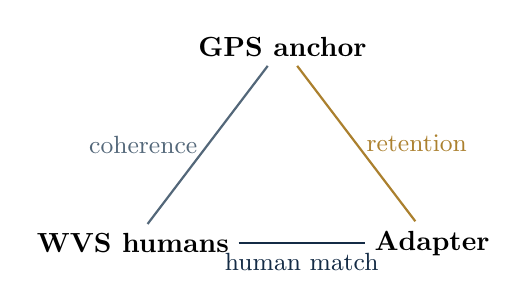
\begin{tikzpicture}[>=Latex]
\node[font=\bfseries] (g) at (0,2.5){GPS anchor};
\node[font=\bfseries] (h) at (-1.9,0){WVS humans};
\node[font=\bfseries] (a) at (1.9,0){Adapter};
\draw[slate,thick] (g)--(h) node[midway,left,font=\small]{coherence};
\draw[gold,thick] (g)--(a) node[midway,right,font=\small]{retention};
\draw[navy,thick] (h)--(a) node[midway,below,font=\small]{human match};
\end{tikzpicture}
\end{column}
\begin{column}{.48\textwidth}
Human--GPS: does this WVS map track GPS.

Adapter--GPS: does the unconditioned policy retain GPS order on new text.

Adapter--human: do policy ranks match people.

A country-named persona is a comparator. It does not receive the sign vector.
\end{column}
\end{columns}
\vspace{2mm}
Held-out synthetic pairs ask a prior question: did fitting recover the imposed labels.
\src{Revised paper §3.3. Two correlations do not establish construct sharing.}
\end{frame}

\begin{frame}{Fitting recovers the imposed labels}
\begin{columns}[T]
\begin{column}{.47\textwidth}{\Huge\color{gold}0.942}

Relative-reward recovery

{\small Chosen--rejected margin improves over the reference.}
\end{column}
\begin{column}{.47\textwidth}{\Huge\color{navy}0.819}

Raw choice accuracy

{\small The adapter itself ranks chosen above rejected.}
\end{column}
\end{columns}
\vspace{3mm}
2,112 held-out country--pair cells. Russia uses a different 132-pair holdout.
\pauseq{What independent test would make this more than a training metric?}
\src{Revised paper §4.1. Recovery is against synthetic labels.}
\end{frame}

\begin{frame}{Anchor retention and human agreement differ}
\begin{center}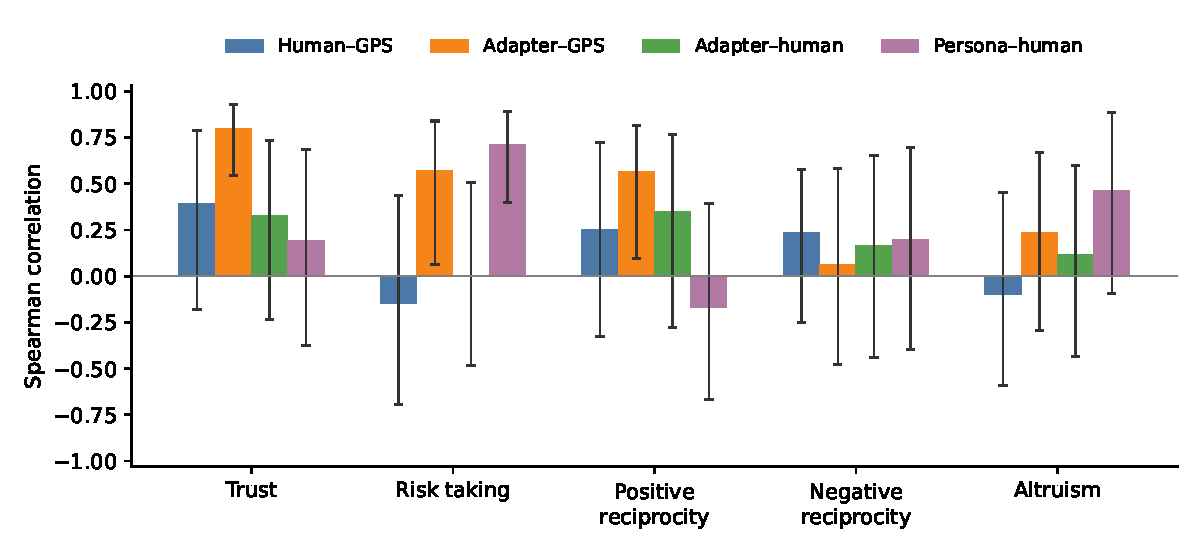
\includegraphics[width=.90\textwidth,height=4.05cm,keepaspectratio]{figures/associations.pdf}\end{center}
{\small Four series, different questions. Risk adapter--human has zero bar height.}
\pauseq{Which association should carry the paper's main empirical claim?}
\end{frame}

\begin{frame}{Trust retains GPS order; human agreement is uncertain}
\begin{center}
\begin{tabular}{@{}lrr@{}}
\toprule
Country-rank association & $\rho$ & 95\% interval\\\midrule
Adapter--GPS & \textbf{0.80} & $[0.55,\ 0.93]$\\[1.2mm]
Persona--GPS & $-0.07$ & $[-0.55,\ 0.45]$\\[1.2mm]
Adapter--human & 0.33 & $[-0.23,\ 0.74]$\\\bottomrule
\end{tabular}
\end{center}
Paired adapter-minus-persona contrast:\quad $0.87\ [0.22,1.36]$.

Permuting GPS trust $z$ across frozen adapter scores, without refitting, gives one-sided $p=0.002$.
\pauseq{Is order-retention on this trust map enough for the contribution?}
\src{Revised paper §4.2. Intervals omit respondent, anchor, and fitting uncertainty.}
\end{frame}

\begin{frame}{A zero on risk does not settle the construct}
\begin{columns}[T]
\begin{column}{.46\textwidth}\textbf{Risk / adapter--human}

{\Huge\color{gold}$\rho=0$}

95\% interval $[-0.48,\ 0.51]$

With 16 countries that interval includes large negative and large positive values. Zero sample rank covariance is not independence of the response distributions, and it is not discriminant validity.
\end{column}
\begin{column}{.50\textwidth}\textbf{Patience / human--GPS}

Q43: work importance\hfill $-0.56$

Q50: financial satisfaction\hfill $+0.62$

We keep the original coding and score the items separately.
\end{column}
\end{columns}
\pauseq{What evidence would separate a bad map from a policy that does not track people?}
\src{Table 4. Q43 interval $[-0.86,-0.04]$; Q50 $[0.11,0.91]$.}
\end{frame}

\begin{frame}{Order and shape need not favor the same configuration}
\begin{center}
\begin{tabular}{@{}lrr@{}}
\toprule
Configuration & Trust--GPS $\rho$ & Mean TVD $\downarrow$\\\midrule
Base / unconditioned & --- & 0.462\\[1mm]
Base / country persona & $-0.07$ & 0.369\\[1mm]
Adapter / unconditioned & 0.80 & 0.480\\[1mm]
Adapter / country persona & 0.67 & 0.401\\\bottomrule
\end{tabular}
\end{center}
The unconditioned adapter keeps the most GPS trust order and is farthest from human response distributions. A country-named base is the reverse.

On risk, adding a country name changes adapter--GPS from 0.57 to $-0.26$. These cells describe configuration sensitivity. They do not identify a general weights-versus-prompts law.
\src{Table 5. TVD averages 368 country--item cells. Isolating route would require giving the prompt the same signs.}
\end{frame}

\begin{frame}{Main contributions of this draft}
\leavevmode\textcolor{gold}{\textbf{1}}\quad An inspectable construction: public GPS signs label a shared pair bank; one joint QLoRA-DPO adapter; country-unconditioned scoring.

\textcolor{gold}{\textbf{2}}\quad An evaluation that keeps recovery, GPS-order transport, and human agreement as separate targets, with a persona comparator on the same items.

\textcolor{gold}{\textbf{3}}\quad Evidence that, on this trust map, unconditioned adapters retain GPS country order more strongly than naming the country, while human ranks and distributional closeness remain unresolved and metric-dependent.

The object is a scoring instrument for group-level item screening. Independent human validation is still required before treating it as a pre-pilot.
\src{Introduction contributions. Not identification of $z$, of a single coordinate, or of culture.}
\end{frame}

\begin{frame}{Open questions before a journal version}
\leavevmode\textcolor{gold}{\textbf{1}}\quad Second scenario bank, same GPS signs, refit two adapters.

\textcolor{gold}{\textbf{2}}\quad Sign-retrain: permute the sixteen sign vectors, relabel, and refit.

\textcolor{gold}{\textbf{3}}\quad Twin-profile exchangeability on held-out WVS.

The assignment permutation in the draft does not refit. Expanding 16 to 24 countries on this bank is later. A blinded human item-screening study is a use-test. It is not compiler identification.
\pauseq{If we can only run one of these before submission, which one?}
\src{Paper 2. Egypt/Q69--Q71 already run: adapter--GPS trust stays 0.79--0.81.}
\end{frame}

\begin{frame}{What would you need to see before using this?}
\bigline{We can inspect the labeling rule and observe trust-order transfer on this panel.}
Human agreement and practical pre-pilot value remain unresolved.

\par\vspace{2mm}
{\Large\color{gold}Discussion}\par\vspace{2mm}

Which part of the construction is least credible?

What evidence would change your view of the proposed use?

Which extension should we run first?
\src{Claim ceiling: group-level scoring instruments intended to complement human survey research.}
\end{frame}

\begin{frame}[t]{Appendix. A complete training pair}
\footnotesize
\noindent\textbf{Scenario.} A fellow student tutored me for free before a critical exam, and now they are facing a tight deadline for their own project and need someone to review their work. Decision: I can either take the time to thoroughly review their project or concentrate on my own study schedule. Trade-off: Helping my fellow student would acknowledge the effort they put into tutoring me, but it would cut into my own study time and potentially impact my performance.

\vspace{1.2mm}
\noindent\textbf{A.} I will set aside time to carefully review their work this evening. They went out of their way to help me when it mattered most, and I want to make sure they know their effort made a difference. If I do not take this seriously, it would feel like I am ignoring the support that helped me succeed.

\vspace{1.2mm}
\noindent\textbf{B.} I will let them know I can only do a quick scan tomorrow morning. My exam prep schedule is already packed with material I have not mastered yet, and I need to be realistic about what I can manage without burning out. I hope they understand my limitations in this situation.

\normalsize
\src{Pair 00023ac74dac. Positive reciprocity. Argentina chooses A. Contractions expanded for typesetting.}
\end{frame}

\begin{frame}{Appendix. Candidate WVS indicators}
\small
\begin{center}
\begin{tabular}{@{}lp{38mm}p{62mm}@{}}\toprule
Anchor & Items & Candidate interpretation\\\midrule
Trust & Q57--Q64, Q73 & Generalized, interpersonal, institutional trust\\[1mm]
Patience & Q43; Q50 & Less work importance; financial satisfaction\\[1mm]
Risk taking & Q106, Q107, Q109, Q178 & Economic values; fare avoidance\\[1mm]
Positive reciprocity & Q81 & Confidence in charitable organizations\\[1mm]
Negative reciprocity & Q176, Q177, Q179, Q195 & Moral clarity; justifiability\\[1mm]
Altruism & Q99, Q101, Q103 & Membership in three types of organizations\\\bottomrule
\end{tabular}
\end{center}
Composites average item means without range standardization. Q57 human--GPS in this panel is 0.15.
\src{Table 2. Strict panel excludes Q69--Q71, Q174, and Q12--Q14.}
\end{frame}

\begin{frame}{Appendix. How we score response codes}
\[
\ell_{cqj}=\sum_t\log\widehat\pi_c(a_{qjt}\mid q,a_{qj,<t}),\qquad
\widehat P_c(j\mid q)=\frac{e^{\ell_{cqj}}}{\sum_h e^{\ell_{cqh}}}
\]
Candidate strings include a leading space. Sum token log probabilities without length normalization; normalize across the supplied codes only.

\[
\text{Item score}=\sum_j g_q(j)\widehat P_c(j\mid q)
\]
Humans use the same recode before a survey-weighted mean. This softmax is a scoring convention. It is not the DPO contest probability.
\src{Revised paper §3.3. Decoder-only model; no sampled response.}
\end{frame}

\begin{frame}{Appendix. Uncertainty, Egypt, mixed-trait bank}
Country bootstrap, 2,000 draws, conditional on the 16 countries, items, and fitted runs. Intervals omit respondent sampling, GPS measurement error, and training randomness.

The shared bank is mixed-trait. Pair loadings are generator judgments. Egypt stays in the primary panel; restoring Q69--Q71 on the other fifteen countries leaves adapter--GPS trust between 0.79 and 0.81.

Still pending for public replay: pinned checkpoint provenance and an isolated calculation from published option probabilities.
\src{Assignment permutation $p=0.002$ on frozen scores. Sign-retrain is unrun.}
\end{frame}

\end{document}
